% !TEX root =  master.tex
\chapter{Umsetzung} \label{umsetzung}
	\section[Organisation]{Organisation{\hfill \normalsize Sandra Keller}}
	\subsection{GitHub}
	GitHub ist ein online System für Software-Entwicklung. Der Name setzt sich zusammen aus Git und Hub. Git ist das zugrunde liegende Versionsverwaltungssystem. Der zweite Teil des Namens \enquote{Hub} ist ein Hinweis auf die Web-Fähigkeiten von GitHub. Dieser Begriff lässt sich als \enquote{zentrale Stelle} oder \enquote{zentraler Sammelpunkt} übersetzen, damit ist der Server gemeint. Das Versionsverwaltungssystem Git kann ohne ein Web-Interface und ohne einen zentralen Server verwendet werden. GitHub reichert die Funktionen von Git jedoch an. Auf der einen Seite hostet GitHub kostenlos OpenSource-Projekte, auf der anderen Seite kann man sich den Entwicklungsprozess mittels grafischer Darstellung im Browser anzeigen lassen. Ein weiterer Vorteil gegenüber Git ist, dass man keinen Kommandozeilen Befehl mehr benötigt, dies kann alles durch einen Mausklick ausgeführt werden. Dies macht GitHub vor allem für Anfänger geeignet. 
	\\GitHub ist dafür bekannt, dass das gemeinsame Arbeiten an Code erleichtert wird. Außerdem ist Problem- und Bug-Tracking integriert und dadurch, dass GitHub von vielen Entwicklern genutzt wird gibt es eine große Datenbank mit verfügbarem Code. Diesen Code kann man praktisch verwenden. So kann man mit Code-Stücken sein Projekt ergänzen und diesen dann anpassen. Ein Entwickler, der eine neue Funktion in sein Projekt einarbeiten will, davor aber zum Beispiel mit der Programmiersprache noch nicht gearbeitet hat, kann auf den Code zugreifen und sich so Hilfe holen. Er kann den Code für sein Projekt anpassen und einbauen. So helfen sich die Nutzer untereinander, es entsteht ein praktischer Wissensaustausch.
	\\Git speichert außerdem jede Version eines Projektes, sollten durch die neuesten Änderungen nicht nur Fehler behoben worden sein, sondern zum Beispiel neue hervorgerufen worden sein, so kann man auf die zurückliegende Version zugreifen.
	
	Innerhalb von GitHub gibt es einige Begriffe mit denen man sich als Anfänger erstmal auseinander setzen muss. 
	Wir haben für unser Projekt ein \enquote{Repository} angelegt, die Dateien von jedem werden darin abgelegt. Innerhalb so eines Repositorys kann es mehrere Versionen einer Software geben, jede Version stellt einen \enquote{Branch} dar. Wenn man eine neue Version eines Branches erstellt hat, weil man etwas am Code verändert hat, so reicht man diese bei der Versionsverwaltung ein, dies nennt man \enquote{commit}. Wenn man als Entwickler einen eigenen Ableger des Repositorys möchte, sodass seine Änderungen nicht direkt in dem original Projekt erscheinen, kann er einen \enquote{Fork} starten. Hier kann der Entwickler privat entwickeln und seine Version am Ende dem ursprünglichen Projekt zuführen. Jedoch kann man auch die eigene Variante weiter bearbeiten und verbreiten.
	\\Git ist mittlerweile in viele Programmierprojekten involviert. Da sich mit Git auch komplexe Projekte managen lassen, es können viele, bis zu tausende Entwickler an einem Projekt arbeiten. Ursprünglich wurde Git dazu entwickelt, um den Linux-Kernel mit einer großen Anzahl an Mitarbeitern zu verwalten und zu verbessern. Durch den einfachen Zugang der Software verbreitete sie sich jedoch sehr schnell auf dem Markt.
	
	Da wir eine Gruppe aus acht Leuten sind, wurde durch GitHub vor allem die Einarbeitung einfacher. Einige hatten schon zuvor mit GitHub gearbeitet, die anderen fanden schnell den besten Weg GitHub zu nutzen. Durch die Bequemlichkeit der grafischen Oberfläche musste man sich keine Konsolenbefehle merken, sondern konnte alles über diese steuern. Des weiteren muss man mit einer so großen Gruppe sehr flexibel sein, das System bietet enorme Flexibilität.
	Auf der anderen Seite gibt es zwar einige Alternativen zu GitHub, diese sind jedoch nicht OpenSource und kosten teilweise sogar für private Nutzer, nicht Unternehmen, einen vierstelligen Preis.
	
	\subsection{IntelliJ IDEA}
	Wir haben uns für die Entwicklungsumgebung IntelliJ IDEA entschieden. Diese wurde von dem Software-Unternehmens JetBrains entwickelt. Sie unterstützt verschiedene Programmiersprachen wie Java, Kotlin, Groovy und Scala. Wir nutzten die OpenSource-Version \enquote{Community Edition}, jedoch gibt es auch eine kostenpflichtige, die \enquote{Ultimate Edition}. Zu den für uns wichtigen Features gehören außerdem die Unterstützung von Apache Maven, JUnit und Tools zur Versionskontrolle, insbesondere Git. Außerdem Code Coverage und auch Test Coverage sind in IntelliJ IDEA integriert. Dieser Versionsumfang kann zusätzlich mit Plug-ins erweitert werden. Diese werden teils von JetBrains, teils von der IntelliJ-Community entwickelt.
	\\Für uns gab es viele Punkte dir für die Nutzung von IntelliJ IDEA gegenüber anderen Entwicklungsumgebungen sprachen. IntelliJ hat eine bessere Konsistenz als Eclipse; alle Editoren und Tools sehen für alle Programmiersprachen gleich aus. Die Editoren für JavaScript, TypeScript, HTML und CSS sind von JetBrains besser ausgearbeitet als die von Eclipse.
	\\IntelliJ IDEA ist außerdem schnell und komfortabel. Die Code-Vervollständigung ist sehr schnell und nutzt auch andere eigene Klasse. Dadurch findet man schneller Fehlerquellen und bekommt meist korrekte Lösungsvorschläge angeboten. Diese muss man anders als bei anderen Entwicklungsumgebungen nicht mit der Maus anklicken sondern sie sind über eine Tastenkombination erreichbar. Eine weitere Erleichterung für Entwickler ist, dass man nie speichern muss, dies passiert automatisch. Dies spart einem nicht nur Zeit, sondern verhindert auch das Vergessen des Speicherns und so Verlust von Daten.
	\\IntelliJ enthält außerdem eine \enquote{Duplicate Code Analyse}, so kann man gleichen Code schnell entdecken und kann den doppelten Code entfernen.
	\\IntelliJ bietet GitHub Support, man kann Projekte direkt in GitHub importieren, man kann seinen Code über einen Knopfdruck in IntelliJ zu dem GitHub Repository hinzufügen, oder sich die neusten Code-Änderungen anzeigen lassen. 
	\\Auch der Datenbank-Support ist bei IntelliJ weit entwickelt. Man kann Datenbankstrukturen visualisieren, in Echtzeit Daten auf der Datenbank ändern oder diese erweitern.
	\\Ein weiteres Feature, dass IntelliJ IDEA gegenüber anderen Entwicklungsumgebungen in den Vordergrund stellt ist die Dokumentation. Diese ist bei vielen Features sehr gut ausgearbeitet und oft sogar mit einem Video unterstützt.
	
	Wir haben uns für IntelliJ IDEA entschieden, da es die ganzen genannten Vorteile birgt und außerdem die Arbeit mit GitHub weiter vereinfacht. Man konnte seinen Code darin schreiben und dem Repository hinzufügen, sich den Code der anderen anschauen und zu dem eigenen Projekt hinzufügen ohne einmal die Umgebung zu verlassen.  So konnten wir unsere Organisations-Elemente effizient nutzen. 
	\\Ein weiterer ausschlaggebender Punkt war, dass wir über IntelliJ alle Daten verarbeitet haben. Die Organisation am Anfang, das codieren des Projektes und auch das Schreiben der Seminararbeit haben wir dort eingearbeitet. Dies war möglich, da wir die Seminararbeit mit LaTeX geschrieben haben.
	
	\subsection{LaTeX}
	LateX ist ein Software-Paket, welches die Benutzung des Textsatzsystems TeX mit Hilfe von Markos vereinfacht. Der Autor arbeitet mit Textdateien, Überschriften und anders zu formatierende Passagen werden mit Hilfe von Befehlen textuell ausgezeichnet. Anders als bei Word, wo man sieht wie der Text am Ende erscheint, sieht man in LaTeX nur die Befehle. Man kann sich jedoch zu jeder Zeit ein PDF ansehen, indem der formatierte Text zu sehen ist. Das Layout ist sehr sauber und auch der Formelsatz sehr ausgereift. Für wissenschaftliche Arbeiten ist LaTeX oft besser geeignet als andere Textverarbeitungssysteme, da es diese komfortablen Möglichkeiten der Formelsetzung gibt. Jedoch muss man sich bevor man mit der Arbeit beginnt erst in die Materie einarbeiten. Dies dauert länger als bei anderen Systemen. Da wir jedoch schon für unsere Projektarbeit LaTeX genutzt haben, war dies für uns nicht entscheidungsrelevant. Für uns standen die Vorteile im Vordergrund.
	\\Als erster Punkt ist hierbei das sogenannte logische Markup zu erwähnen. Überschriften zum Beispiel werden nicht nur mit Fettdruck gekennzeichnet, sondern auch als Überschrift. So wird ein Inhaltsverzeichnis generiert, das man nicht selbst anlegen muss. So auch bei Quellenangaben oder bei einem Abbildungsverzeichnis.
	\\LaTeX ist weitestgehend rechnerunabhängig verwendbar. Es gibt für die meisten Betriebssysteme produktiv einsetzbar LaTeX-Installationen. Ein weiterer Vorteil besteht darin, dass das Ergebnis unabhängig vom Rechner und dem verwendeten Drucker die Formatierung exakt gleich ist. LaTeX ist zum Beispiel nicht an die Schriftarten eines Rechners gebunden.
	\\Für alle Sachen, die komplizierter sind als bei anderen Textverarbeitungssystemen ist außerdem eine sehr aktive Gemeinschaft da, es gibt besonders im wissenschaftlichen Bedarf für alles Ergänzungen.
	
	\section[Backend]{Backend{\hfill \normalsize Martin Sandig}}
\subsection{Grundgerüst}\label{umsetzung:backend:grundgeruest}
--> Komponentendiagramm erstellen



Das Backend wurde anhand des Fachkonzeptes implementiert. Da die grundlegende Anforderung für dieses, die Umsetzung in Java ist, wurde hierzu ein Java-Projekt mit Maven aufgesetzt. Apache Maven ist ein Software-Projektmanagement- und Verständniswerkzeug.\autocite{ApacheSoftwareFoundation} Es dient unter anderem dazu, den Aufbau von Projekten zu definieren, benutzte Frameworks zentral zu organisieren sowie einen Projektlebenszyklus abzubilden. Der in Maven implementierte Lebenszyklus umfasst mehrere Stadien, welche sich vom \glqq Clean\grqq, also dem Aufräumen eines Projektes, über \glqq Test\grqq \, bis zum \glqq Install\grqq \, bzw. \glqq Deploy\grqq \, erstrecken. Zwischen diesen Stadien existieren noch viele mehr, welche für diese Seminararbeit keine Rolle spielen sollen. Am Ende des \glqq Install\grqq -Stadiums steht eine ausführbare JAR-Datei zur Verfügung.

Die Konfiguration von Maven wird in einem \ac{POM} definiert. Hierzu existiert eine \glqq pom.xml\grqq-Datei im \ac{ICS}-Projekt. Die eigentliche Umsetzung des Backendes erfolgte mit Hilfe des \glqq Spring\grqq -Frameworks. Spring ist ein Framework, welches für die Entwicklung von Java-Projekten vereinfachen soll sowie ein breites Spektrum an Funktionalitäten für Geschäftslogiken mitliefert.  Genauer gesagt beruht das Backend auf \glqq Spring-Boot\grqq, welches ein Bestandteil des Spring-Frameworks ist. Es dient dazu eigenständig lauffähige Spring-Anwendungen zu entwickeln, wobei alle nötigen Bibliotheken mitgeliefert werden.\autocite{PivotalSoftwareInc} In diesem Fall handelt es sich um eine Spring-Boot-Webanwendung. Für die Konfiguration des \ac{POM} gibt es vordefinierte Templates, sogennante \glqq Archetypes\grqq. Aus diesen heraus lässt sich ein Maven-Projekt generieren, welches alle nötigen Basiseinstellungen mitbringt. Einen solcher Archetype existiert auch für Spring-Boot-Anwendungen, welcher für das \ac{ICS}-Projekt genutzt wurde.

Das Spring-Framework arbeitet mit Hilfe von \ac{IoC}-Containern. \ac{IoC} ist ein Prinzip bei der Software-Entwicklung, bei der man die Steuerung der Anwendung bzw. die Steuerung von Objekten auf einen Container bzw. an ein Framework übertragen wird. Die \ac{IoC}-Container im Spring-Framework arbeiten nach dem \ac{DI}-Konzept, bei dem Abhängigkeiten von Objekten behandelt werden. Durch dieses Konzept müssen Objekte ihrer Abhängigkeiten nicht selber suchen sondern bekommen die benötigten Ressourcen bzw. Abhängigkeitsobjekte vom Framework zugewiesen. (QUELLE) Der \ac{IoC}-Container, welcher in diesem Projekt genutzt wurde nennt sich \glqq Application-Context \grqq. Objekte, welche sich in diesem Container bzw. Kontext befinden werden \glqq Spring Beans\grqq \, genannt. Spring Beans können auf verschiedene Arten deklariert und initiiert werden. Im Fall dieses Projektes werden alle benötigten Spring Beans beim Starten der Anwendung initiiert. Die Deklaration der Beans erfolgt zum einen durch Java-Annotations innerhalb von Java-Klassen. Zum Anderen werden die Beans in einer Konfigurationsdatei des Application-Contextes definiert. Diese Datei nennt sich \glqq applicationContext.xml\grqq.

Um nun die Spring-Boot-Anwendung ausführbar zu machen wurden zwei Klassen, siehe Quelltext \ref{lst:IcsApplication} und \ref{lst:IcsWebConfiguration} angelegt. Innerhalb der \glqq IcsApplication\grqq -Klasse wird mit Hilfe der Annotation \glqq @SpringBootApplication\grqq \, und dem Inhalt der \glqq main-Methode\grqq \, definiert, dass es sich um eine Spring-Boot-Anwendung handelt. Die Klasse \glqq IcsWebConfiguration\grqq \, dient zur erweiterten Konfiguration der Spring-Boot-Anwendung. Durch die Annotation \glqq @Configuration\grqq \, und die Implementierung des \glqq WebMvcConfigurer\grqq -Interface wird dem Spring-Framework mitgeteilt, dass es sich hierbei um eine Konfigurationsklasse handelt, welche beim Starten der Anwendung berücksichtigt werden muss. Durch die Annotation \glqq @ImportResource(...)\grqq \, wird die Konfigurationsdatei für den Application-Context geladen.

\lstset{language=Java}
\begin{lstlisting}[caption={IcsApplication.java}, label={lst:IcsApplication}]
@SpringBootApplication
@EnableAutoConfiguration
@EnableScheduling
public class IcsApplication {
public static void main(String[] args) {
SpringApplication.run(IcsApplication.class, args);
}
}
\end{lstlisting}

\lstset{language=Java}
\begin{lstlisting}[caption={IcsWebConfiguration.java}, label={lst:IcsWebConfiguration}]
@Configuration
@ImportResource("classpath:spring/applicationContext.xml")
public class IcsWebConfiguration implements WebMvcConfigurer {
/**Something more **/
@Override
public void addResourceHandlers(ResourceHandlerRegistry registry) {
if (System.getProperty("os.name").contains("Windows")) {
registry
.addResourceHandler("/content/**")
.addResourceLocations("file:///".concat(
ApplicationEnvironment.getContentPath()
.toString().concat("/")));
} else {
registry
.addResourceHandler("/content/**")
.addResourceLocations("file://".concat(
ApplicationEnvironment.getContentPath()
.toString().concat("/")));
}
}
}
\end{lstlisting}

Da es sich beim \ac{ICS}-Projekt um eine Webanwendung handelt wurde in der \glqq IcsWebConfiguration\grqq -Klasse, siehe Quelltext \ref{lst:IcsWebConfiguration}, ein weiterer \glqq ResourceHandler\grqq \, hinzugefügt, welcher einen \glqq content\grqq-Ordner auf dem Dateisystem zu einer URL (\glqq localhost:8080/content/*\grqq) der Webanwendung zuordnet. Dieser Ordner dient als Ablage für anzuzeigende Bilder der späteren Webseite. Damit dieser Ordner auf dem Dateisystem vorhanden ist, wurde ein Klasse \glqq FileSystemInitilizer\grqq \, implementiert. Beim Start der Anwendung wird ein Spring-Bean dieser Klasse initiiert, welches eine Ordnerstruktur auf dem Dateisystem anlegt. Hierfür ist es möglich eine Umgebungsvariable für die Anwendung zu setzten. Sollte diese nicht gesetzt worden sein, wird stattdessen der \glqq tmp\grqq- Ordner auf dem Root-Verzeichnis des Betriebssystems als Ausgangsordner für die Dateistruktur der Anwendung verwendet bzw. gegebenenfalls angelegt.

Dadurch, dass Spring selbstständig Einstellungen für die Webanwendung vornimmt war es nicht nötig weitere Konfigurationen für eine Webanwendung vorzunehmen. Beispielsweise verbindet Spring automatisch einen \glqq public\grqq Ordner im Projekt mit der laufenden Webanwendung. Innerhalb dieses Ordners werden alle Dateien abgelegt (HTML, JavaScript, CSS), welche zum Anzeigen der Website relevant sind.

\subsection{Datenbank} \label{umsetzung:backend:datenbank}
Für die \ac{ICS}-Anwendung wurde beschlossen eine Datenbank als Persistenz-Schicht zu verwenden. Das Schema dieser wurde anhand des ER-Modells aus der Entwurfsphase (ER DIA!!!!) entwickelt. Hierzu wurde ein Java-Framework namens \glqq Liquibase\grqq \, verwendet.\autocite{Liquibase} Liquibase ist ein Framework zum Verfolgen, Verwalten und Anwenden von Datenbankschemaänderungen, welches unabhängig von der zugrundeliegenden Datenbank arbeitet. Das Framework arbeitet mit einem sogenannten \glqq Database-Changelog\grqq, in welchem die Änderungshistorie des Datenbankschemas festgehalten wird. Der Changelog wird in einer XML-Struktur festgehalten. Die Änderungshistorie setzt sich aus \glqq ChangeSet\grqq-Einträgen zusammen, welche mit einen eindeutigen \ac{ID} und dem Autor gekennzeichnet werden. Ein Beispiel bzw. ein Auszug des ChangeLog's der \ac{ICS}-Anwendung ist in Quelltext \ref{lst:dbChangelog} zu sehen.

\lstset{
	language=XML,
	morekeywords={encoding,databaseChangeLog,changeSet,column,constraints,createTable,addColumn,modifyDataType,xs:schema,xs:element,xs:complexType,xs:sequence,xs:attribute,xsi:schemaLocation,xmlns:xsi,xmlns}
}
\begin{lstlisting}[caption={Database-Changelog Liquibase}, label={lst:dbChangelog}]
<databaseChangeLog
xmlns="http://www.liquibase.org/xml/ns/dbchangelog"
xmlns:xsi="http://www.w3.org/2001/XMLSchema-instance"
xsi:schemaLocation="http://www.liquibase.org/xml/ns/dbchangelog   
http://www.liquibase.org/xml/ns/dbchangelog/dbchangelog-3.1.xsd">

<changeSet id="1" author="martin">
<createTable tableName="Payment_Method">
<column name="pay_uuid" type="varchar(255)">
<constraints primaryKey="true" nullable="false" unique="true"/>
</column>
<column name="provider" type="varchar(255)">
<constraints nullable="false"/>
</column>
<column name="pay_description" type="varchar(255)">
<constraints nullable="true"/>
</column>
</createTable>
</changeSet>
</databaseChangeLog>
\end{lstlisting}

Der Database-Changelog, siehe Quelltext \ref{lst:dbChangelog}, wird bei jedem Starten der Anwendung mit der zugrundeliegenden Datenbank verglichen. Neue Änderungen bzw. neue ChangeSets, werden anschließend auf der Datenbank angewandt. Hierin liegt auch der große Vorteil von Liquibase. Wechselt man die Datenbank im Hintergrund, so muss man keinen großen Aufwand betreiben, die Datenbank einzurichten. Sollte das Datenbankschema beim Starten der Anwendung nicht mehr mit der Änderungshistorie übereinstimmen, so werden zum Schutz der Anwendung der Startvorgang unterbrochen und entsprechende Fehlermeldungen erzeugt.

\begin{figure}[H]
	\centering 
	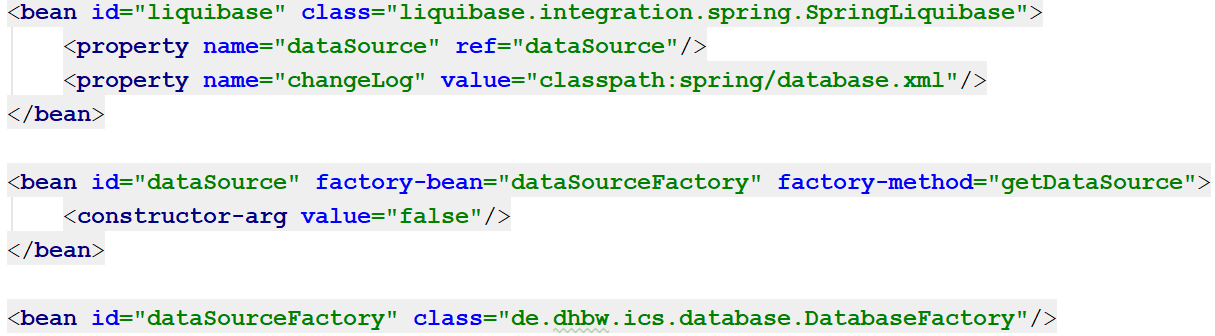
\includegraphics[width=0.8\textwidth]{img/liquibase_beans}
	\captionsetup{format=hang}
	\caption[Spring-Konfiguration für Liquibase]{\label{fig:liquibase_spring}Spring-Konfiguration für Liquibase}
\end{figure}

Ein weiterer Vorteil von Liquibase ist, dass es eine Integration für das Spring-Framework, siehe Kapitel \ref{umsetzung:backend:grundgeruest}, mit sich bringt. Hierfür wurden mehrere Spring-Beans definiert, welche in Abbildung \ref{fig:liquibase_spring} zusehen sind. Wie man in dieser Abbildung erkennen kann, hängt das Bean für Liquibase (mit der \ac{ID} \glqq liquibase\grqq) von zwei Parametern ab. Der Parameter \glqq changelog\grqq \, gibt den Pfad zur Datei für die Konfiguration bzw. der Änderungshistorie an. Der zweite Parameter \glqq dataSource\grqq \, hat als Übergabewert eine Referenz zu einem anderen Spring-Bean. Dieses Bean liefert ein \glqq DataSource\grqq-Objekt zurück welches in der Klasse \glqq DataSourceFactory\grqq erzeugt wird. Diese DataSource enthält die Verbindungsdaten für die Datenbankverbindung. Im aktuellen Release des \ac{ICS}-Projektes sind die Verbindungsdaten noch nicht parametrisiert, sondern fest im Code implementiert. Für einen späteren Auslieferungs-Release würden die Verbindungsdaten, wie URL, Passwort und Benutzername über Umgebungsvariablen setzbar sein.

Als Standard-Datenbank für die \ac{ICS}-Anwendung wurde eine H2-Datenbank verwendet. Die H2-Datenbank ist eine leichtgewichtige, in Java entwickelte Datenbank.\autocite{H2} Der Vorteil dieser ist, dass sie sehr einfach aufgebaut ist, zur Laufzeit angelegt oder bei Bedarf auch in Memory erzeugt werden kann. Im Fall von \ac{ICS} wird eine H2-Datenbank beim erstem Starten der Anwendung in dem Ordner \glqq database\grqq, welcher sich in der Dateistruktur der Anwendung befindet, angelegt. Dieser Ordner wird von dem im Kapitel \ref{umsetzung:backend:grundgeruest} erwähnten \glqq FileSystemInitializer\grqq \, erstellt, falls dieser noch nicht vorhanden ist.

\subsection{Fachkonzept}

Das Fachkonzept wurde anhand des Entwurfs, siehe Kapitel \ref{entwurf}, entwickelt. Hierzu wurde sich an verschiedenen Entwicklungskonzepten orientiert und bzw. an diese angelehnt. Ein Beispiel hierfür ist \ac{DDD}. \ac{DDD} ist ein von Eric Evans geprägter Begriff, welcher eine Herangehensweise an die Modellierung komplexer Software beschreibt. \autocite{WikimediaFoundationInc.2019a}

\subsubsection{Anbindung der Datenbank}

Um die einzelnen Entitäten der Datenbank im Backend zu verwirklichen, wurde ein zu den Entwurfsmustern des \ac{DDD}, nämlich der \glqq Value-Objects\grqq \, bzw. der Entity-Objects, ähnliches Verfahren angewandt. Value-Objects zeichnen sich damit aus, dass sie keine Identität besitzen und sich nur durch ihre Eigenschaften definieren. Entity-Objects hingegen werden nicht durch ihre Eigenschaften sondern anhand ihrer Identität definiert. \autocite{WikimediaFoundationInc.2019a} Im Fall von \ac{ICS} wurde eine Vermischung dieser beiden Muster angewandt, da sich die Objekte zum einen durch ihre Identität aber auch durch ihre Eigenschaften definieren (Aggregate). Für jede Entität bzw. Tabelle der Datenbank wurde eine eigene Klasse (folglich genannt Entitätenklasse) angelegt. Diese Klassen, wie zum Beispiel \glqq User\grqq , \glqq Room \grqq , oder \glqq Presentation\grqq wurden im \glqq de.dhbw.ics.vo\grqq-Paket des \ac{ICS}-Projektes angelegt.

Der nächste Schritt der Anbindung der Datenbank an das Backend war die Implementierung von sogenannten \ac{DAO}'s. Das \ac{DAO} ist ein Entwurfsmuster, welches den Zugriff auf unterschiedliche Arten von Datenquellen verwirklicht. \autocite{WikimediaFoundationInc.2019b} Für jede Entitätenklasse wurde eine \ac{DAO}-Klasse angelegt, welche die typischen \ac{CRUD}-Methoden implementieren. Hierfür wurde ein Interface \glqq Dao\grqq \, deklariert, welches alle \ac{CRUD}-Methoden beinhaltet, siehe Abbildung \ref{fig:dao_klassendia}. Dieses Interface wird von der abstrakten Klasse \glqq AbstractDao\grqq \, implementiert, jedoch wurden die Methoden des Interfaces abstrakt gelassen. Die abstrakte Klasse beinhaltet allgemeine Methoden um die \ac{CRUD}-Operationen auf der Datenbank ausführen zu können. Die Kind-Klassen, wie beispielsweise \glqq SeatDao\grqq, rufen diese Methode mit den für ihre Entität spezifischen Parametern in der \ac{CRUD}-Methode (bspw. \glqq persist\grqq) auf. Sollte die verallgemeinerten Methoden des AbstractDao für eine Entität nicht ausreichend sein, so wurden sie innerhalb der DAO-Klassen der Entitäten überschrieben.

\begin{figure}[H]
	\centering 
	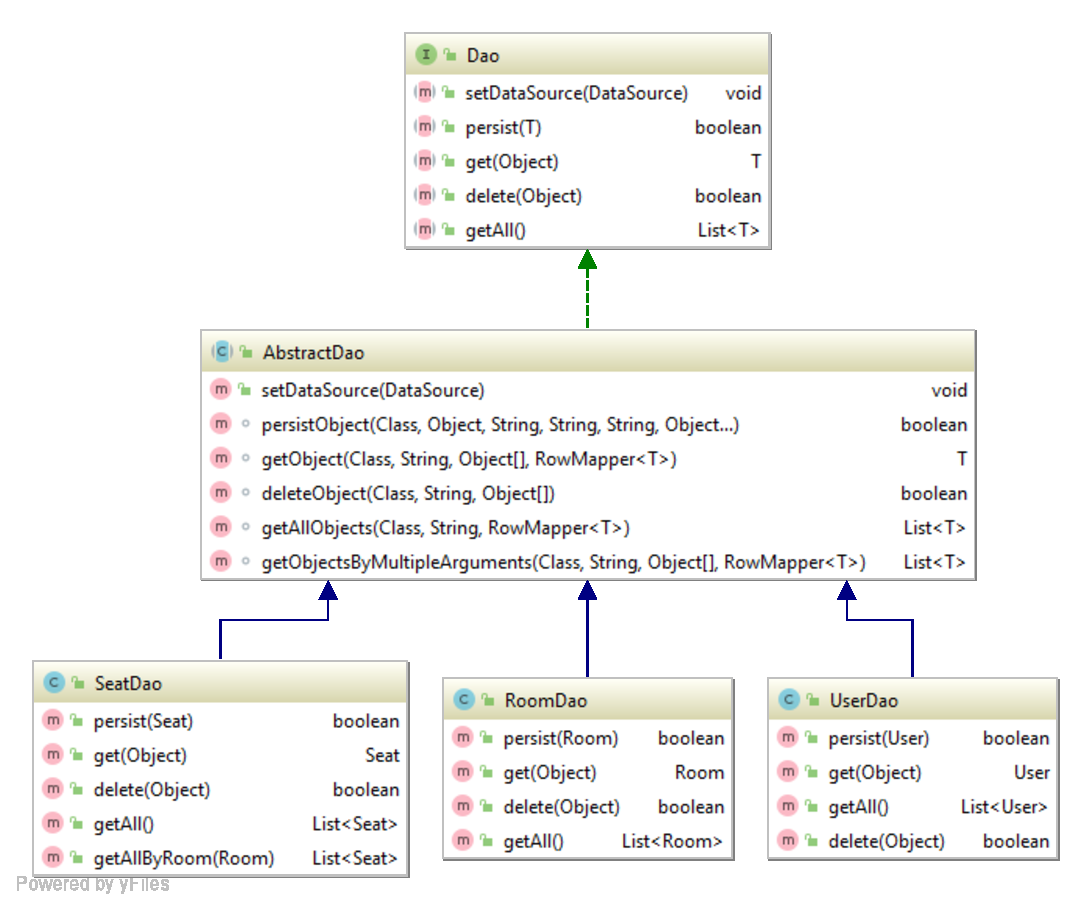
\includegraphics[width=0.8\textwidth]{img/dao_klassendia}
	\captionsetup{format=hang}
	\caption[Ausschnitt Klassendiagram \ac{DAO}-Vererbungshierarchie]{\label{fig:dao_klassendia}Ausschnitt Klassendiagramm \ac{DAO}-Vererbungshierarchie}
\end{figure}

Der eigentliche Zugriff auf die Datenbank bzw. das Ausführen von Operationen auf der Datenbank wurde durch \ac{JDBC}-Templates realisiert. \ac{JDBC} ist eine Datenbankschnittstelle für relationale Datenbanken, welches von durch die JAVA-Plattform zur Verfügung gestellt wird. \autocite{WikimediaFoundationInc.2019c} Spring bietet hierfür verschiedene Templates an, welche das Arbeiten mit JDBC vereinfachen.\autocite{PivotalSoftwareInc.b} 

\begin{figure}[H]
	\centering 
	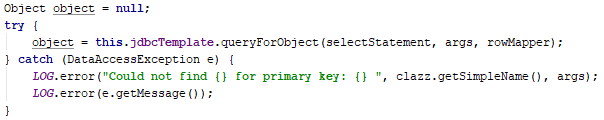
\includegraphics[width=0.8\textwidth]{img/jbdc_template_usage}
	\captionsetup{format=hang}
	\caption[\ac{JDBC}-Template-Verwendung]{\label{fig:jbdc_template_usage}\ac{JDBC}-Template-Verwendung}
\end{figure}

Ein Beispiel für die Implementierung ist in Abbildung \ref{fig:jbdc_template_usage} zu sehen. Das \ac{JDBC}-Template bietet für beispielsweise \glqq SELECT\grqq-Abfragen eigene Methoden wie \grqq queryForObject\grqq. Dieser Methode müssen nur ein SQL-Befehl mit fehlenden Parametern, die Argumente bzw. Parameter für den SQL-Befehl sowie ein \glqq RowMapper\grqq-Objekt übergeben werden, um ein Objekt auf der Datenbank abzufragen. Die fehlenden Argumente der übergebenen SQL-Anweisungen, welche durch einen ?-Operator markiert sind, siehe Abbildung \ref{fig:select_beispiel}, werden innerhalb des \ac{JDBC}-Templates durch die übergebenen Argumente ergänzt. 

\begin{figure}[H]
	\centering 
	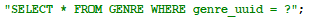
\includegraphics[width=0.5\textwidth]{img/select_beispiel}
	\captionsetup{format=hang}
	\caption[Beispiel einer SQL-Anweisung für \ac{JDBC}]{\label{fig:select_beispiel}Beispiel einer SQL-Anweisung für \ac{JDBC}}
\end{figure}

Das \ac{JDBC}-Template wird durch die Übergabe einer DataSource erzeugt. Hierfür wurde die gleiche DataSource verwendet, welche auch für die Initiierung von Liquibase verwendet wurde. Hierzu wurden von allen  \ac{DAO}-Klassen Spring-Bean Deklarationen angelegt sowie eine \glqq Set-Methode\grqq für die DataSource angelegt, siehe Abbildung \ref{fig:dao_klassendia} und \ref{fig:dao_spring}.

\begin{figure}[H]
	\centering 
	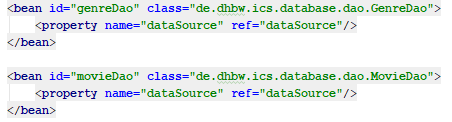
\includegraphics[width=0.8\textwidth]{img/dao_spring}
	\captionsetup{format=hang}
	\caption[Beispiel für die Spring-Bean-Deklaration von \ac{DAO}-Objekten]{\label{fig:dao_spring}Beispiel für die Spring-Bean-Deklaration von \ac{DAO}-Objekten}
\end{figure}	

Der letzte Schritt der Anwendung war die Implementierung von Mapper-Klassen, welche die Ergebnisse der Datenbankabfrage in Entitäten umwandeln bzw. Objekte dieser Erzeugen. Hierfür stellt Spring das bereits erwähnte Interface RowMapper zur Verfügung. 

\subsubsection{Fach-Logik}

Das Fachkonzept der \ac{ICS}-Anwendung wurde innerhalb von den Klassen \glqq PresentationManager\grqq und \glqq ReservationManager\grqq umgesetzt. Diese Manager werden ebenfalls als Spring-Bean deklariert, siehe Kapitel \ref{umsetzung:backend:grundgeruest}. Weiterhin bilden die Manager eine Verwaltungsschicht vor der Datenbankschicht, sprich vor den \ac{DAO}-Objekten. Da aus diesem Grund die Manager mit den \ac{DAO}-Objekten arbeiten, wurden private Attribute für jedes genutzte \ac{DAO} angelegt, siehe Abbildung \ref{fig:manager_dao}. Diese Attribute bzw. Objekte werden mit Hilfe des Spring-Frameworks bzw. des ApplicationContextes, siehe Kapitel \ref{umsetzung:backend:grundgeruest}, gesetzt, welches durch die Annotation \glqq Autowired\grqq \, signalisiert wird. 

\begin{figure}[H]
	\centering 
	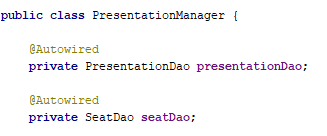
\includegraphics[width=0.5\textwidth]{img/manager_dao}
	\captionsetup{format=hang}
	\caption[Beispiel für die \ac{DAO}-Attribute der Manager]{\label{fig:manager_dao}Beispiel für die \ac{DAO}-Attribute der Manager}
\end{figure}	


Der PresentationManager dient zur Verwaltung von Prozessen, welche mit dem Bearbeiten und Anzeigen von Vorstellungen zu tun haben. Im aktuellen Release bietet dieser Manager folgende Funktionalitäten an:

\begin{itemize}
	\setlength\itemsep{-0.5em}
	\item Auflisten von allen Preiskategorien
	\item Auflisten aller Vorstellungen
	\item Auflisten aller Vorstellungen innerhalb eines Zeitintervalls
	\item Auflisten aller Vorstellungen für einen bestimmten Film in einem Zeitintervall
	\item Auflisten aller Vorstellungen nach einem bestimmten Suchstring
	\item Persistieren neuer Vorstellungen
	\item Löschen von Vorstellungen
	\item Ausgabe einer bestimmten Vorstellung
	\item Auflisten aller Filme
	\item Auflisten aller Filme nach einem bestimmten Titel-Suchstring
	\item Auflisten aller Filme in einem bestimmten Zeitintervall
\end{itemize}

Dabei wurde darauf geachtet, dass innerhalb der für diese Funktionalitäten zur Verfügung stehenden Methoden Überprüfungen der Übergabeparameter eingearbeitet wurden. Beispielsweise ist es nicht möglich eine Vorstellung zu persistieren, welche keinen zugewiesenen Raum oder Film besitzt oder in der Vergangenheit liegt.

Der ReservationManager basiert auf dem gleichen Konzept, wie der PresentationManager. Er dient dazu alle Prozesse abzudecken, welche das Reservieren von Sitzplätzen umfassen. Im derzeitigen Release des \ac{ICS}-Projektes existiert noch kein Manager für die Benutzerverwaltung. Aus diesem Grund wurden im ReservationManager vorerst auch Funktionalitäten einer Benutzerverwaltung implementiert. Beispielsweise ist es möglich einen Benutzer bzw. Gast-Benutzer zu überprüfen sowie neue anzulegen. Weitere wichtige Funktionalitäten des ReservationManagers sind: 

\begin{itemize}
	\setlength\itemsep{-0.5em}
	\item Persistieren einer Reservierung
	\item Löschen einer Reservierung
	\item Sperren und Entsperren von Sitzen im Reservierungsprozess
\end{itemize}

Der Reservierungsprozess ist in Abbildung /*****/ dargestellt. Ein wichtiger Bestandteil bei diesem ist das Sperren von Sitzen für andere Benutzer. Die Sperrwirkung für Sitze wurde im ReservationManager umgesetzt. Hierfür wurden zwei Methoden implementiert (\glqq lock\grqq \, und \glqq unlock\grqq) , siehe Quelltext \ref{lst:lockProcess}. Der Sperrprozess funktioniert folgender Maßen:

Nachdem ein Anwender Sitze einer Vorstellung im Frontend ausgewählt hat und anschließend auf den Button zum Starten des Reservierungsprozesses betätigt hat, wird eine Liste mit den ausgewählten Sitzen, die Vorstellungs-\ac{ID}, eine Session-\ac{ID} sowie ein Parameter, welcher bestimmt ob die Sitze gesperrt oder entsperrt werden sollen, an das Backend geschickt. Anschließend wird die Liste sowie die angegeben Vorstellungs-\ac{ID} überprüft. Beispielsweise wird überprüft, ob die Sitze auch zur angegeben Vorstellen passen bzw. ob diese überhaupt vorhanden sind. Sofern die Überprüfung erfolgreich ist beginnt danach der Sperrprozess. Bei diesem wird überprüft, ob es dem Client erlaubt ist, die Sitze zu sperren. Dies erfolgt mittels der Session-ID, welche beim ersten Aufruf der Anwendung generiert und dem Client als Cookie mitgegeben wird. Innerhalb der Datenbank existiert eine Tabelle namens \glqq BusySeat\grqq, welche den aktuellen Zustand eines Sitzes für eine Vorstellung repräsentiert. Aus dieser Tabelle heraus werden Entitäten-Objekte erstellt, welche folgende Attribute besitzen: \glqq Seat, Presentation, isBusy, isLocked, sessionID, timestamp\grqq. Das Attribute isBusy sagt aus, dass ein Sitz bereits belegt ist. In diesem Fall ist es also nicht mehr möglich einen Sitz zu sperren. Das Attribute isLocked repräsentiert, ob ein Sitz gerade gesperrt ist. Befindet sich also ein Sitz in einem gesperrten Zustand, so wird durch das Attribute sessionID der Client ausgewiesen, welcher ihn gesperrt hat und durch das Attribute timestamp, wann er dies getan hat. Möchte nun ein Client einen Sitz sperren, so wird zunächst geprüft ob ein Eintrag in der Tabelle BusySeat vorhanden ist. Ist dies nicht der Fall so kann der Sitz gesperrt werden. Sollte ein Eintrag vorhanden sein, so wird die Session-ID überprüft. Stimmt die Session-ID in der Datenbank mit der des Client überein, so kann der Sitz ebenfalls gesperrt werden. Ansonsten wird überprüft ober der angegeben Zeitstempel älter ist als 5 min. Wenn er älter ist, so kann der Datenbankeintrag überschrieben und der Sitz gesperrt werden. Nachdem alle Sitze die Überprüfung bestanden haben, werden sie in der Datenbank gespeichert. Sollte beim Speichervorgang ein Fehler auftreten oder nicht alle Sitze die Überprüfung bestanden haben so wird dem Client ein Fehler zurück gegeben. Der selbe Prozess erfolgt bei der Entsperrung der Sitze.

Des Weiteren wurde mit Hilfe von Spring ein \glqq Scheduling-Task\grqq \, implementiert, welcher alle 5min die BusySeat-Tabelle überprüft und alle gesperrten Entitäten, welche einen Zeitstempel besitzen der 5min in der Vergangenheit liegt, entsperrt.

\lstset{language=Java}
\begin{lstlisting}[caption={Implementierung zum Sperren von Sitzen}, label={lst:lockProcess}]
private Object lockSeats(List<Seat> seats, String sessionID, Presentation presentation) {
List<BusySeat> bsUpdate = new ArrayList<>();
for (Seat s : seats) {
BusySeat bs = getBusySeat(presentation, s);
if (bs != null) {
if (bs.isBusy())
return ResultMessage.SEAT_TAKEN;

if (bs.isLocked() && !bs.getSessionID().equals(sessionID)) {
int offset = BusySeat.compareLockTimestamp(bs);
if (offset > 0) {
return ResultMessage.LOCKED_SEAT;
}
}

bs.setBusy(false);
bs.setLocked(true);
bs.setSessionID(sessionID);
bs.setTimestamp(Calendar.getInstance().getTimeInMillis());
s.setCurrentBusySeat(bs);
s.addBusy(bs);
continue;
}

bs = new BusySeat(false, s, presentation, true, sessionID, Calendar.getInstance().getTimeInMillis());
bsUpdate.add(bs);
s.setCurrentBusySeat(bs);
s.addBusy(bs);
}
if (bsUpdate.size() == seats.size()) {
if (this.busySeatDao.persistBatch(bsUpdate)) {
return seats;
}
}
return ResultMessage.COULD_NOT_BLOCK_SEATS;
}

private Object unlockSeats(List<Seat> seats, String sessionID, Presentation presentation) {
List<BusySeat> bsUpdate = new ArrayList<>();
for (Seat s : seats) {
BusySeat bs = getBusySeat(presentation, s);
if (bs != null) {
if (bs.isBusy())
return ResultMessage.SEAT_TAKEN;

if (bs.isLocked() && bs.getSessionID().equals(sessionID)) {
bs.setLocked(false);
bs.setTimestamp(0);
bs.setSessionID("");
bsUpdate.add(bs);
s.setCurrentBusySeat(bs);
s.addBusy(bs);
}
}  
}
if (bsUpdate.size() == seats.size()) {
if (this.busySeatDao.persistBatch(bsUpdate)) {
return seats;
}
}
return null;
}

\end{lstlisting}

\subsection{REST-Schnittstellen}

Für den dynamischen Datenaustausch zwischen Front- und Backend wurde sich dazu entschlossen \ac{REST}-Schnittstellen zu verwenden. \ac{REST} bezeichnet ein Programmierparadigma für verteilte Systeme, welches sich an dem Verhalten des \ac{WWW} orientiert.\autocite{REST} Im Fall von \ac{ICS} wurden \ac{REST}-Schnittstellen entwickelt, welche mit dem HTTP-Protokoll arbeiten und mit \ac{JSON}-Objekten umgehen können. Hierfür bietet Spring, siehe Kapitel \ref{umsetzung:backend:grundgeruest}, die Möglichkeit einfache sogenannte \glqq RestController\grqq zu implementieren, siehe Abbildung \ref{fig:beispiel_restcontroller}.

\begin{figure}[H]
	\centering 
	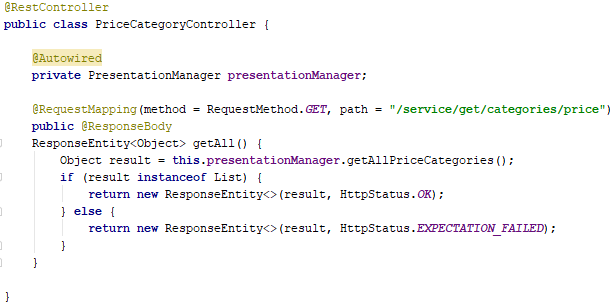
\includegraphics[width=\textwidth]{img/beispiel_restcontroller}
	\captionsetup{format=hang}
	\caption[Beispiel für einen RestController]{\label{fig:beispiel_restcontroller}Beispiel für einen RestController}
\end{figure}	

	
	\section[Frontend]{Frontend {\hfill \normalsize Jonas Dutzi, Dennis Köhler}}
	
	\subsection{Responsive Merkmale}
	Ziel des Projektes sollte es ebenfalls sein die Kinowebseite nicht nur für den großen Bildschirm am Computer zu entwickeln, sondern auch die Darstellung auf gegebenenfalls kleineren Endgeräten zu beachten. Die Nutzung von Websites auf mobilen Geräten steigt seit einigen Jahren kontinuierlich an. Im Jahr 2018 wurden zum Beispiel 52,2\% aller Aufrufe von Webseiten von Smartphones durchgeführt, während im Jahr 2009 noch nicht einmal 1\% aller Aufrufe durch die mobilen Geräte abgedeckt war\footnote{https://www.statista.com/statistics/241462/global-mobile-phone-website-traffic-share/}. Das zeigt auf wie wichtig das Thema des Responsive Webdesigns ist und welche Rolle es noch in der Zukunft spielen wird. Um diejenigen Nutzer, welche die Kinowebsite auch auf mobilen Endgeräten verwenden wollen nicht mit schlecht dargestelltem Inhalt zu enttäuschen, wurden in diesem Projekt hauptsächlich zwei Elemente des Bootstrap Frameworks zur Hilfe gezogen. Zum einen das Gitter System für die Anzeige von Inhalten und zum anderen die sich einklappende Navigationsleiste.
	
	Das in Bootstrap vorhandene Gitter System macht es möglich Inhalte, welche in Tabellenform bzw. in Reihen und Spalten, angezeigt werden an verschiedene Gerätegröße anzupassen. Hierfür werden drei vorgefertigte CSS-Klassen verwendet. Das äußere Div erhält die Klasse \texttt{.container} und umspannt den gesamten Inhalt. Innerhalb dieses Containers können Reihen und Spalten angelegt werden, welche durch weitere Divs mit den Klassen \texttt{.row} (Reihe) und \texttt{.col} (Spalte) realisiert werden. Diese kann man nach seinen Bedürfnissen schachteln, um die gewünschte Anzahl an Reihen und Spalten zu realisieren. Durch die Erweiterung \texttt{.col-\# (\# = 1-12)} kann die Breite und Anzahl der Elemente pro Reihe genau definiert werden. Hierbei stelle 12 die gesamte Seitenbreite dar, welche zum Beispiel mit einem 
	\texttt{col-12}  Element, zwei \texttt{col-6} Elementen oder drei \texttt{col-4} Elementen gefüllt werden kann. Um zu erreichen, dass bei variierender Gerätegröße unterschiedlich viele Elemente pro Reihe angezeigt werden, kann der Zusatz \texttt{.col-xx-\#}hinzugefügt werden. An stelle von xx kann nun eine vorgefertigten Gerätegrößen gewählt werden:
	
	\begin{table}[H]
		\centering
		\begin{tabular}{p{3,5cm} | c | c }
			\textbf{Klasse} & \textbf{Gerätegröße} & \textbf{Pixel} \\\toprule
			.col-xs-\# &  Extra small &  bis 576 \\
			.col-sm-\# &  Small &  bis 768  \\
			.col-md-\# &  Medium &  bis 922  \\
			.col-lg-\# &  Large &  bis 1200  \\
			.col-xl-\# &  Extra large &  über 1200  \\
		\end{tabular}
		\caption[Gerätegrößen]{\label{tab:gerätegrößen}Gerätegrößen }
	\end{table}
	
	Das Spalten-Div kann zu jeder Größe eine eigene Klasse mit definierter Breite implementieren. Am Beispiel der Filmkacheln der Startseite wird die Verwendung deutlich:
		\begin{center}
			<div class=“col-sm-12 col-md-6 col-lg-4”>
		\end{center}

	Bei kleinen Geräten wird die volle Breite (12) ausgenutzt und eine Kachel nimmt die gesamte Reihe ein. Übersteigt die Gerätegröße 768px teilen sich zwei Kacheln die volle Breite (6+6), ab 922px werden drei Kacheln nebeneinander angezeigt (4+4+4).
	
	Ein weiteres sich anpassendes Element stellt die Navigationsleiste dar. Ziel ist es bei kleineren Gerätegröße nicht den gesamten Inhalt anzuzeigen, sondern ihn hinter einem Button zu verstecken. Bei Betätigung dieses Buttons soll der Inhalt in Form einer Dropdown-Liste angezeigt werden. Um dies zu erreichen ist innerhalb des \texttt{<nav> </nav>} - HTML-Tags ein Button zu erstellen, welchem die in Bootstrap vorgefertigte CSS-Klasse \texttt{.navbar-toggler} zugewiesen wird. Die einzuklappenden Inhalte werden Innerhalb eines Divs, welches die vorgefertigten Klassen \texttt{.collapse}, \texttt{.navbar-collapse}, sowie eine feste ID besitzt, definiert. Diese ID wird dann dem Button-Attribut \texttt{data-target} zugewiesen. Zuletzt wird über die Klasse \texttt{.navbar-\\expand-lg} definiert, dass die Navigationsleiste ab einer Fenster-/Gerätebreite von kleiner als 992 Pixel hinter dem Button verschwindet. Die Abbildungen \vref{fig:navLeiste} und \vref{fig:navLeisteAus} zeigen das Ergebnis:
	\begin{figure}[H]
		\centering 
		
\includegraphics[width=13cm]{img/navLeiste.png}
		\captionsetup{format=hang}
		\caption[Navigationsleiste]{\label{fig:navLeiste} Navigationsleiste auf Geräten\\ mit einer Breite von über 992 Pixeln}
	\end{figure}
	
	\begin{figure}[H]
		\centering 
		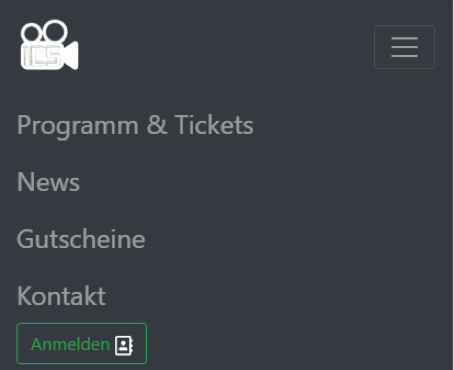
\includegraphics[width=6cm]{img/navLeisteAus.png}
		\captionsetup{format=hang}
		\caption[Navigationsleiste ausgeklappt]{\label{fig:navLeisteAus} Navigationsleiste ausgeklappt auf dem Smartphone (Breite 414 Pixel)}
	\end{figure}

	\subsection{Design}
	Um Nutzer anzuziehen und deren Erwartungen an eine moderne Website gerecht zu werden sollte das Ergebnis nicht nur funktional und responsive sein, sondern auch gut aussehen. Hierfür wurde bereits im Vorfeld der Umsetzung ein Design Entwurf angefertigt (Kapitel \vref{design}), welcher die Struktur vorgeben sollte. Diese wurde bei der Entwicklung auch weitestgehend eingehalten und es fanden neben der Umgestaltung der Navigationsleiste hauptsächlich kleinere Veränderungen, wie die Verschiebung von Inhalten statt. Einige Merkmale wurden im Entwurf jedoch noch nicht aufgeführt bzw. berücksichtigt und wurden erst während des Entwicklungsprozesses entschieden. 
	
	
	Einen wichtigen Punkt hierbei stellt die Farbwahl dar. Aufgrund der großen Beliebtheit, die die sogenannten \enquote{Darkmodes} neuer Betriebssystemversionen, Webseiten oder Apps mit sich bringen wurde auch für die Kinowebseite ein eher dunkleres Farbschema gewählt. Diese haben neben der subjektiven Einschätzung der Nutzer auch technische Vorteile wie die Entlastung der Augen in dunkleren Umgebungen oder geringeren Energieverbräuchen auf Endgeräten mit OLED-Display\footnote{https://www.futurezone.de/produkte/article215761243/Deshalb-bist-du-als-Android-User-mit-dem-Dark-Mode-im-Vorteil.html}. Um die Website einheitlich und nicht zu bunt zu gestalten wurde Grün als Akzentfarbe gewählt.
	
	
	Weitere unterschiede zum Entwurf sind in der Navigationsleiste erkennbar. Der Entwurf sieht eine zweizeilige Leiste mit getrennten, als Button gestalteten Schaltflächen vor. Bei der Betrachtung anderer Webseiten fiel jedoch auf, dass zum einen zweispaltige Navigationsleisten eher vermieden werden und zum anderen fließende Übergänge zwischen den Inhalten moderner wirken als durch Linien getrennte Bereiche. In Folge dessen wurde die Navigationsleiste in der \ac{ICS}-Webseite einzeilig und als ein zusammenhängender Bereich implementiert. Das Hervorheben der Schaltflächen geschieht durch die farbliche Aufhellung der entsprechenden Überschrift. 
	
	
	Das Hervorheben von Inhalten geschieht über die Webseite verteilt jedoch auf verschiedene Arten. Neben der erwähnten Aufhellung, kommen verschiedene Mauszeiger (Cursor) zum Einsatz. Den in HTML definierten Bereichen kann mithilfe des Cursor Attributs ein geeignetes Aussehen für den Mauszeiger zugeordnet werden. Inhalte die einen Link darstellen werden typischerweise mit dem \texttt{pointer}-Cursor versehen, welcher eine zeigende Hand symbolisiert. Neben diesem findet zum Beispiel der \texttt{not-allowed}-Cursor bei bereits belegten Sitzen des Sitzplans Verwendung. Eine weitere Möglichkeit des Hervorhebens ist bei den Filmkarten auf der Startseite verwendet worden. Diese beginnen bei Berührung des Cursors eine kleine Animation, welche durch ein JS-Script realisiert wurde und die gesamte Karte nach oben hebt. 
	
	Ein weiteres Designelement stellt der Slider dar. Dieser könnte beim Einsatz für ein Kino neben aktuellen Filmen auch Angebote oder spezielle Events werben. Auch wenn Kritiker Slider als nebensächlichen oder platzverschwendenden Inhalt ansehen und Studien die Ineffektivität der erreichten Werbewirkung darstellen\footnote{https://www.contentconsultants.de/blog/webdesign-slider-sind-out-weg-damit/} wurde sich bewusst dafür entschieden. Hierzu trugen die subjektiven Einschätzungen der Entwickler sowie der Ist-Vergleich zu anderen Kinowebseiten, siehe Kapitel \vref{istAnalyse}, bei.
	
	Zuletzt ist noch der Sitzplan zu erwähnen. Dieser wurde mithilfe des in %TODO 6.3.1 
	beschriebenen Frameworks erstellt und soll die Auswahl der zu reservierenden Sitze möglichst einfach und intuitiv gestalten. Der Saal wird als Menge von kleinen Quadraten, welche die Sitze darstellen, angezeigt. Bereits reservierte Sitze werden transparent grau, freie Sitze in grün eingefärbt. Der Nutzer kann die gewünschten Plätze durch Anklicken auswählen und gegebenenfalls durch erneutes Klicken abwählen. Abbildung \vref{fig:sitzplan} zeigt den Sitzplan in der finalen Version.
	
	\begin{figure}[H]
		\centering 
		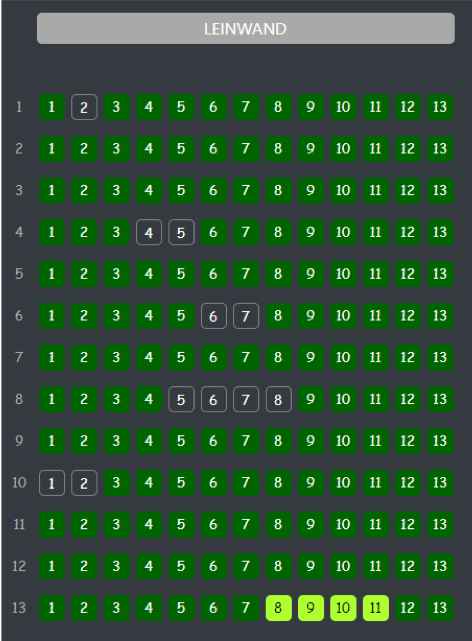
\includegraphics[width=9cm]{img/sitzplan.png}
		\captionsetup{format=hang}
		\caption[Sitzplan]{\label{fig:sitzplan} Sitzplan (Ausgewählte Sitze: 8,9,10,11 in Reihe 13)}
	\end{figure}

	\subsection{Ablauf des Bestellvorgangs}
	
	
	\section[Verknüpfung Back- und Frontend]{Verknüpfung Back- und Frontend {\hfill \normalsize Sandra Keller}}
	REST

	
	\section[Modultests]{Modultests{\hfill \normalsize Fabio Westphal}}
	Das Testen von Code stellt einen essenziellen Teil der Entwicklung von Software dar. Der ANSI/IEEE Standard 610.12-1990 definiert Tests folgendermaßen:	\enquote {An activity in which a system or component is executed under specified conditions, the results are observed or recorded, and an evaluation is made of some aspect of the system or component.} Man unterscheidet grundsätzlich Whitebox- und Blackbox-Tests. Bei Whitebox-Tests wird die innere Funktionsweise der Software getestet, wohingegen bei Blackbox-Tests kein Wissen über den Quellcode zugrundeliegt und nur der geforderte Funktionsumfang getestet wird.\autocite{franz2007handbuch}[Vgl.][S.28] Im Projekt wurden hauptsächlich Komponententests angewendet, welche zu den Whitebox-Tests zählen. Hierbei werden Klassen und Methoden einzeln parallel zur weiteren Entwicklung getestet. Durch die kleinschrittige Testweise tragen sie auch zur lebenden Dokumentation bei. Wichtig ist dabei, dass jeder Test korrekt,
schnell, abgeschlossen,	isoliert, sprechend benannt, wartbar und einfach durchführbar
ist.
	Es muss der gesamte Code einmal durchlaufen werden, um maximale Korrektheit zu sichern.\autocite{witte2015testmanagement}[Vgl.][S.50] Bei überschauberen Systemen kann man aber auch nur kritische Teile testen. Um die Tests automatisiert auszuführen, werden Test-Frameworks verwendet. In diesem Projekt wird das bekannte Framework JUnit benutzt.
	Bei Datenbankzugriffsklassen ist es vor allem wichtig, die \ac{CRUD}-Operationen zu testen. Diese gelten als die essenziellen Funktionen, wenn es um den Zugriff auf Datenbanken geht. Im Projekt wurde dafür die Klasse \texttt{DaoTestHelper} verwendet, die entsprechende Schnittstellen für die Testklassen zur Verfügung stellt. Im Zuge eines Tests werden zunächst Beispielobjekte erzeugt und persistiert. Anschließend werden die Grundoperationen mithilfe der Helper-Klasse getestet. Am Beispiel der Klasse \texttt{MovieDaoTest} sieht das wie folgt aus:
	\begin{lstlisting}
public class MovieDaoTest {

	private static Movie movie;
	private static Genre genre;
	
	@Autowired
	private GenreDao genreDao;
	
	@Autowired
	private MovieDao movieDao;
	
	@BeforeClass
	public static void setUp() throws Exception {
		movie = new Movie(2015, "TestMovie", "Nice Test Movie", 12, 120);
		genre = new Genre("testGenre");
		movie.setGenre(genre);
	}
	
	@Test
	public void test1Persist() {
		assertFalse(this.movieDao.persist(movie));
		assertTrue(this.genreDao.persist(genre));
		DaoTestHelper.persist(this.movieDao, movie);
	}
	
	@Test
	public void test2Get() {
		DaoTestHelper.get(this.movieDao, movie, movie.getUuid());
	}
	
	@Test
	public void test3GetAll() {
		DaoTestHelper.getAll(this.movieDao, movie);
	}
	
	@Test
	public void test4Update() {
		Movie testMovie = new Movie(movie.getUuid(), 2000,"updatedMovie", movie.getDescription(), movie.getFsk(), movie.getRunTime());
		testMovie.setGenre(movie.getGenre());
		DaoTestHelper.update(this.movieDao, movie.getUuid(), movie, testMovie);
	}
	
	@Test
	public void test5Delete() {
		DaoTestHelper.delete(this.movieDao, movie.getUuid());
	}
}
	\end{lstlisting}
	Beim Ausführen der Tests gibt es in der Entwicklungsumgebung IntelliJ die Möglichkeit, die Abdeckung zu berechnen. Dabei werden zum einen die Zeilen gezählt, die von den Tests betroffen sind und zum anderen die Methoden bzw. Klassen. In Relation zur Gesamtheit der Zeilen - bzw. Methoden oder Klassen - ergibt dies die Testabdeckung als Prozentzahl (siehe Abb. \ref{fig:TestCoverage}).\newline
	\begin{figure} 
		\centering 
		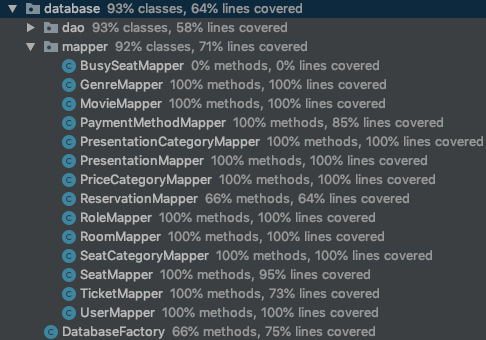
\includegraphics[scale=0.6]{img/testCoverage.png}
		\captionsetup{format=hang}
		\centering\caption[Testabdeckung]{\label{fig:TestCoverage} Übersicht der Testabdeckung}
	\end{figure}
	Die Testabdeckung ist häufig ein faktisches Kriterium für die Qualität des Codes bei Abnahme des Projekts. Beim Erreichen einer bestimmten Prozentzahl fällt allerdings auf, dass diese beim Schreiben der Tests nicht linear steigt. Das liegt daran, dass viele Klassen, die explizit getestet werden, Methoden anderer Klassen wie beispielsweise Superklassen oder Helper-Klassen nutzen. Somit werden diese direkt auch getestet. Andere Klassen wiederum verwenden genau die gleiche Superklasse (oder Helper-Klasse...), die bereits zuvor fremdgetestet wurde. Es sind also weniger Zeilen Code, die für die Testabdeckung zählen, obwohl ähnlich viele Zeilen durchlaufen werden. Daher ist es in der Regel der Fall, dass bei den ersten Tests die Testabdeckung stark wächst, dann jedoch immer langsamer.
	
	
	\section[Ausblick]{Ausblick {\hfill \normalsize Milena Zahn}}\label{Ausblick}
	%\subsection{Lessons Learned} 
	Die Bereiche, an denen gearbeitet wurde, waren vielfältig. Zuerst waren alle an der Analyse sowie der Erarbeitung des Entwurfs beteiligt. Dann musste sich das Team erarbeiten, wie ein solches Projekt umgesetzt werden kann. Die Programmierung des Backends war für einige der Teammitglieder komplett neu, aber da das Team sehr unterschiedliche Fähigkeiten besitzt, war dies in der geplanten Projektzeit möglich. Auch die Erstellung des Frontends war eine interessante Erfahrung. Die Verbindung von diesem mit dem Backend war für die meisten von uns eine weitere Herausforderung, da in diesem Bereich noch wenige Erfahrungen gemacht wurden. 
	Neben dem technischen Wissen haben die Teammitglieder auch einige weitere Kompetenzen in dem Projekt erworben. Eine davon ist, dass es sehr wichtig ist, andere Projekte, an denen die Teammitglieder außerhalb des Moduls arbeiten müssen, bei dem Projektplans zu berücksichtigen. Obwohl dies sehr schwierig ist, kann dies helfen, den Projektplan genauer und realistischer zu erstellen. Es ist sehr wichtig, für jede Aufgabe genügend Zeit einzuplanen, um unerwartete Herausforderungen zu bewältigen. Die selbständige Erarbeitung von Vorgehensweisen und Lösungskonzepte ist eine weitere in diesem Projekt erworbene Kompetenz.
	Eine weitere Hürde war die Gruppengröße von acht Personen. Es ist schwierig das Potenzial der Gruppe voll ausschöpfen, weil die Arbeit innerhalb der Gruppe gut organisiert werden muss.  Um eine übermäßige Koordination der Mitglieder und lange Kommunikationswege zu vermeiden, haben wir die Gruppe in Untergruppen mit verschiedenen Aufgabenbereichen aufgeteilt. Somit konnte eine schnelle Entscheidungsfindung und kurzfristige Absprachen garantiert werden. Insgesamt wurden in der engen Projektzeit viele unterschiedliche Kompetenzen erworben und vor allem die theoretischen Inhalte der Vorlesung Systemanalyse angewandt.
	